\documentclass[a4paper,12pt]{article}
\addtolength{\oddsidemargin}{-1.cm}
\addtolength{\textwidth}{2cm}
\addtolength{\topmargin}{-3cm}
\addtolength{\textheight}{3.5cm}
\makeindex


\usepackage[pdftex]{graphicx}
\usepackage{makeidx}
\usepackage{float}
\usepackage{hyperref}
\hypersetup{
	colorlinks=true,
	linkcolor=blue,
	filecolor=magenta,      
	urlcolor=cyan,
}



% define the title
\author{CodeBlox}
\title{Tender}
\begin{document}
	\setlength{\parskip}{6pt}
	
	% generates the title
	\begin{titlepage}
		\begin{center}
			
\includegraphics[width=1\textwidth]{./Pictures/up_logo.png}\\[1.5cm] 
			\textsc{\LARGE Department of Computer Science} \\ [.5cm]
			\textsc{\Large Functional and Architectural Requirements} \\ [.5cm]
			\line(1,0){450}\\[.5cm]
			\huge{\bfseries Client: Gavin Potgieter}\\
			\line(1,0){450}\\[.5cm]
			\textsc{\LARGE Team: CodeBlox}\\ [0.5cm]
			
			
			\textsc{\large Tshepo Malesela (Bsc: Computer Science)}\\
			\textsc{\large Lorenzo Spazzoli (Bsc: Computer Science)}\\
			\textsc{\large Bilal Muhammad (BIS: Multimedia)}\\
			\textsc{\large Dirk de Klerk (BIS: Multimedia)}\\ [3.9cm]
			
			\large\today
		\end{center}
	\end{titlepage}
	
	\tableofcontents
	\thispagestyle{empty}
	\footnotesize
	\normalsize
	
	
	
	
	\newpage
	\section{Introduction}
	The purpose of this document is to provide a detailed overview of the functional and architectural requirements with regard to the DropOff Project that was assigned to team CodeBlox. The document will be under constant revision, and will change as the project progresses. 
	
	{\noindent}It will provide the development team with a reference that can be used to develope from, thus ensuring that all functional and architectural requirements are met.
	
	{\noindent}The document will also serve as means of communication between the client and development team. Thus any additional requirements from the clients' side can be appended to the document, and has to be adhered to from the development side.
	
	\section{Project Objectives} The \textbf{primary objective} of the project is to create an automated service system that will provide customers with the ability to grant delivery personnel access to a drop safe and/or demarcated area of their home. This will ensure that deliveries to be made can be completed without the need of someone being physically present on the premises.
	
	{\noindent}Initially this will consist of the generation of a One Time Pin (OTP), that will be sent to the delivery personnel, granting them single access to the demarcated area. Once the delivery has been made. The user needs to be able to ensure that the residence is secure.
	
	{\noindent}If time allows it. The system will be expanded to use audio and video communication to validate the identity of the delivery person.
	
	{\noindent}In addition to the functionality of the system, it needs to be as \textbf{cost effective} as possible. This will allow a larger audience to gain access to the system. 
	
	{\noindent}The \textbf{secondary objective} (if time permits) is to make the system scalable. This will enable services to expand to other areas of the home. Thus allowing users an affordable solution to home automation.
	
	\newpage
	\section{Functional Requirements}
	
	\subsection{PersonService}
	The PersonService module will be responsible for maintaining user information. The module will also have the responsibility of storing demographic information about the users, store information about the users' next of kin, and finally keep track of the users account status.
	
	\subsubsection{Scope}
	The scope of the Users module is shown below
	
	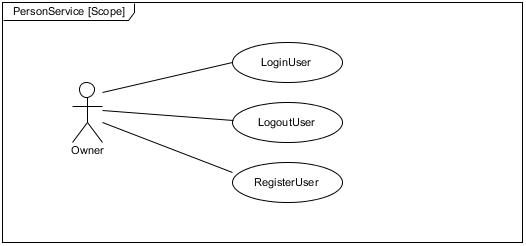
\includegraphics[width=1\textwidth]{./Pictures/UML/Usecase/PersonServiceUseCase.jpg}\\[0cm]
	
	{\noindent}The scope of the Users module includes
	\begin{itemize}
		\item adding, removing, and modifying users on the system
		\item changing user information
	\end{itemize}
	
	\subsubsection{Domain Model}
	The domain model for the Users module is shown below
	
	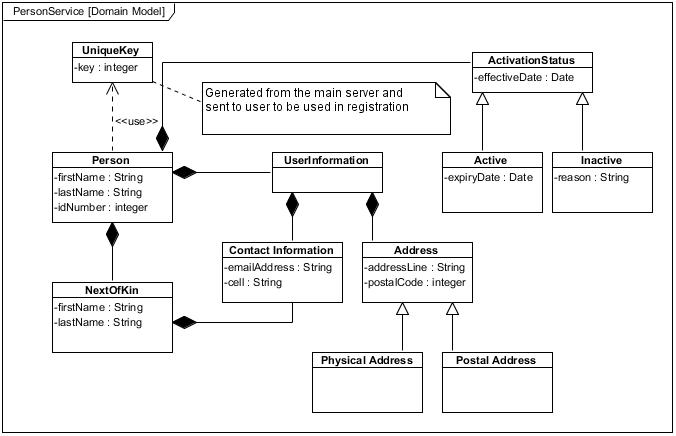
\includegraphics[width=1\textwidth]{./Pictures/UML/PersonServiceDomain.jpg}\\[1.5cm]	

	{\noindent}Each user has a firstname and a lastname, as well as an id number. Each person will also have associated with them UserInformation, which will include email, cellphone, as well as Address. A next of kin will also be available in case the user cannot be reached. Lastly the Person will have associated with it an ActivationStatus, that will determine if the user is still able to receive services.	
	 
	\newpage
	\subsubsection{Use Cases}
	
	\begin{itemize}
		\item \textbf{loginUser} - Allows a user to log into the system.\\[0.5cm]
		\textit{preconditions:}
			\begin{itemize}
				\item The user has already been registered with the system.
				\item The user is still considered an active user.
				\item The user has provided the correct login credentials.
			\end{itemize}
			
		\textit{postconditions:}
			\begin{itemize}
				\item The user is logged into the system.
				\item User gains access to all the services available to him/her.\\[0.5cm]
			\end{itemize}
			
		\item \textbf{logoutUser} - Allows a user to logout of the system.\\[0.5cm]
		\textit{preconditions:}
			\begin{itemize}
				\item The user is already logged into the system.
			\end{itemize}
		
		\textit{postconditions:}
			\begin{itemize}
				\item The user is logged out of the system.
				\item The user no longer has access to the services provided by the system.\\[0.5cm]
			\end{itemize}
			
		\item \textbf{registerUser} - Allows a user to be registered on the system and provide them access to the various services.\\[0.5cm]
		\textit{preconditions:}
			\begin{itemize}
				\item The user does not already exist on the system.
				\item The user has been provided with a unique registration key
			\end{itemize}
		
		\textit{postconditions:}
			\begin{itemize}
				\item The user has been added to the system and may continue.\\[0.5cm]
			\end{itemize}
			
		\item \textbf{updateDetails} - Allows a user to update their information.\\[0.5cm]
		\textit{preconditions:}
			\begin{itemize}
				\item The user exists on the system
				\item The user has to correct credentials
			\end{itemize}
		
		\textit{postconditions:}
			\begin{itemize}
				\item The users' information is updated.
			\end{itemize}
	\end{itemize}
	
	\newpage
	
	\subsection{CameraService}
	The CameraService is responsible for providing the user with access to the live camera feed. The user needs to be able to access a feed, and also needs to be able to close a camera feed. This will ultimately allow them to verify the identity of the delivery person. 
	
	\subsubsection{Scope}
	The scope of the CameraService module is shown below
	
	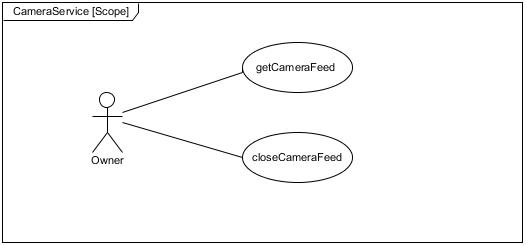
\includegraphics[width=1\textwidth]{./Pictures/UML/Usecase/CameraServiceUseCase.jpg}\\[0cm]
	
	{\noindent}The scope of the CameraService module includes
	\begin{itemize}
		\item Gaining access to the live camera feed.
		\item Close the camera feed as a means to save on bandwidth.
	\end{itemize}
	
	\subsubsection{Domain Model}
	The domain model for the CameraService module is shown below
	
	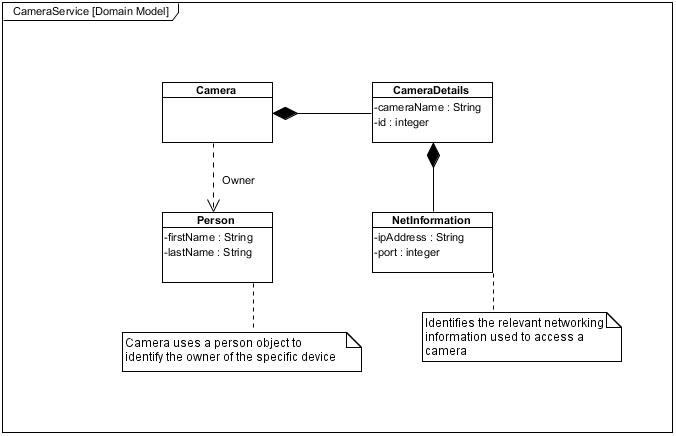
\includegraphics[width=1\textwidth]{./Pictures/UML/CameraServiceDomain.jpg}\\[1.5cm]	
	
	{\noindent}Each Camera will have associated with it CameraDetails that will provide information to how the camera may be accessed. Also the Camera Class will be associated with a Person class to identify them as the owner of the device.
	
	\newpage
	\subsubsection{Use Cases}
	
	\begin{itemize}
		\item \textbf{getCameraFeed} - Enables the user to gain access to the live camera feed.\\[0.5cm]
		\textit{preconditions:}
		\begin{itemize}
			\item The user is still active in the system.
			\item The camera is available to be accessed.
		\end{itemize}
		
		\textit{postconditions:}
		\begin{itemize}
			\item The user receives a live stream.\\[0.5cm]
		\end{itemize}
		
		\item \textbf{closeCameraFeed} - Allows a user to close a camera feed.\\[0.5cm]
		\textit{preconditions:}
		\begin{itemize}
			\item The camera feed is currently streaming.
		\end{itemize}
		
		\textit{postconditions:}
		\begin{itemize}
			\item The camera stops streaming a live feed.\\[0.5cm]
		\end{itemize}
	\end{itemize}
	
	\newpage
	\subsection{PinService}
	The PinService Module is responsible for generating new pins as a backup, should the camera system fail. The module will also need to keep track of the status of the pin i.e. whether or not it has been used or not, as well as its life time. If a pin has been used or it has reached its life time maximum, a new pin has to be generated.
	
	\subsubsection{Scope}
	The scope of the PinService module is shown below
	
	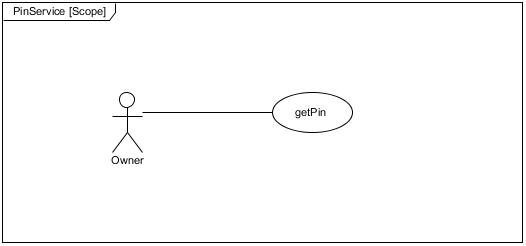
\includegraphics[width=1\textwidth]{./Pictures/UML/Usecase/PinServiceUseCase.jpg}\\[0cm]
	
	{\noindent}The scope of the PinService module includes
	\begin{itemize}
		\item Generating a new pin.
		\item Keeping track of a pins' validity through life time and status.
	\end{itemize}
	
	\subsubsection{Domain Model}
	The domain model for the PinService module is shown below
	
	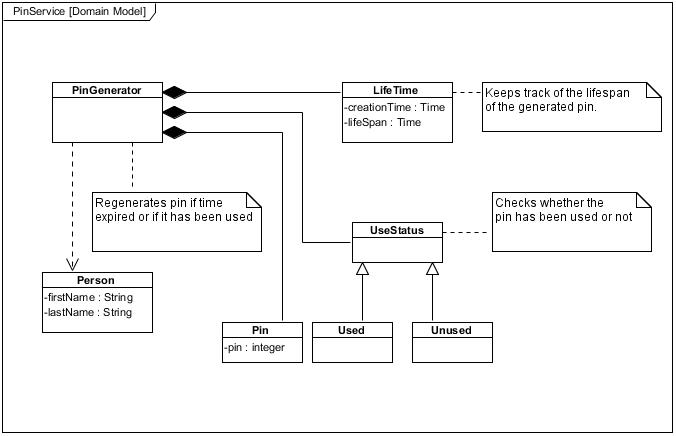
\includegraphics[width=1\textwidth]{./Pictures/UML/PinServiceDomain.jpg}\\[0cm]	
	
	{\noindent}The main class will be the PinGenerator. Associated with each pin generator will be a Pin, which will store the relevant pin that may be used as a fail safe. Also associated with the PinGenerator are the LifeTime and UseStatus classes, which are responsible for monitoring the Pins' validity. The PinGenerator is also associated with a Person so that each generated pin is sent to the correct person.
	
	\newpage
	\subsubsection{Use Cases}
	
	\begin{itemize}
		\item \textbf{generatePin} - The System will generate a new pin to be used as a fail safe.\\[0.5cm]
		\textit{preconditions:}
		\begin{itemize}
			\item A pin has expired.
			\item A pin has already been used.
		\end{itemize}
		
		\textit{postconditions:}
		\begin{itemize}
			\item A new pin is generated.\\[0.5cm]
		\end{itemize}
		
		\item \textbf{displayKeypad} -  The keypad to enter the pin will be displayed.\\[0.5cm]
		\textit{preconditions:}
		\begin{itemize}
			\item The system is making use of the failsafe.
		\end{itemize}
		
		\textit{postconditions:}
		\begin{itemize}
			\item The keypad is displayed on screen.\\[0.5cm]
		\end{itemize}
		
		\item \textbf{updateServer} -  The pin is updated server side for later use.\\[0.5cm]
		\textit{preconditions:}
		\begin{itemize}
			\item A new pin has been generated.
		\end{itemize}
		
		\textit{postconditions:}
		\begin{itemize}
			\item The new pin is reflected on the server.\\[0.5cm]
		\end{itemize}
		
		\item \textbf{getPin} - Allows the user to receive the generated pin.\\[0.5cm]
		\textit{preconditions:}
		\begin{itemize}
			\item The user is logged into the system.
			\item The pin is available.
		\end{itemize}
		
		\textit{postconditions:}
		\begin{itemize}
			\item The pin is sent to the user.\\[0.5cm]
		\end{itemize}
	\end{itemize}
	\newpage
	
	\subsection{LockService}
	The LockService Module will have the responsibility of controlling access to the dropbox. The lock mechanism can be comprised of any suitable technology for example a step motor or magnetic lock. The service should be able to unlock and lock the device, as well as keep track of the device status.
	
	\subsubsection{Scope}
	The scope of the LockService module is shown below
	
	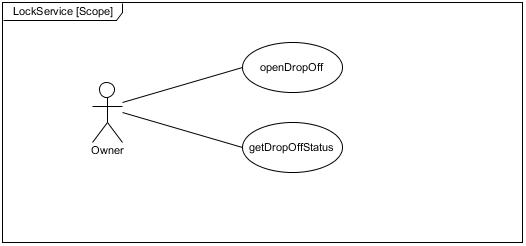
\includegraphics[width=1\textwidth]{./Pictures/UML/Usecase/LockServiceUseCase.jpg}\\[0cm]
	
	{\noindent}The scope of the LockService module includes
	\begin{itemize}
		\item Open up the dropOff box (via unlock or rotate of motor)
		\item Lock the dropOff box
		\item keep track of the devices' status.
	\end{itemize}
	
	\subsubsection{Domain Model}
	The domain model for the LockService module is shown below
	
	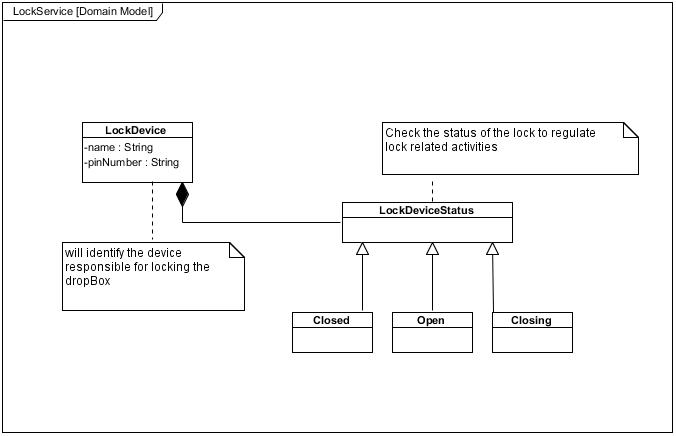
\includegraphics[width=1\textwidth]{./Pictures/UML/LockServiceDomain.jpg}\\[0cm]	
	
	{\noindent}The LockDevice Class consists of a name and a pinNumber. The name is used to identify the device and pinNumber will be used to identify the pin used to interface with the raspberry pi. Associated with the LockDevice class will be a LockDeviceStatus, that will be used to keep track of the devices' current status i.e. Closed, Open, and Closing.
	
	\newpage
	\subsubsection{Use Cases}
	
	\begin{itemize}
		\item \textbf{openDropOff} - Will allow the user to open up the box once identity has been verified.\\[0.5cm]
		\textit{preconditions:}
		\begin{itemize}
			\item The box is closed.
			\item The user is logged in.
			\item The camera feed is accessible (System is functioning normally).
		\end{itemize}
		
		\textit{postconditions:}
		\begin{itemize}
			\item The box is opened up.\\[0.5cm]
		\end{itemize}
		
		\item \textbf{lockDropOff} -  This function will allow the dropOff box to be locked and secured again.\\[0.5cm]
		\textit{preconditions:}
		\begin{itemize}
			\item The device is currently open/unlocked.
		\end{itemize}
		
		\textit{postconditions:}
		\begin{itemize}
			\item The device is locked.\\[0.5cm]
		\end{itemize}
		
		\item \textbf{getDropOffStatus} -  Provides the user/system with state information about the system.\\[0.5cm]
		\textit{preconditions:}
		\begin{itemize}
			\item The system is in some state, either Open, Closed, Closing.
		\end{itemize}
		
		\textit{postconditions:}
		\begin{itemize}
			\item The appropriate state is returned to the system/user.\\[0.5cm]
		\end{itemize}
	\end{itemize}
	\newpage
	
	\subsection{NotificationService}
	The NotificationService Module is responsible for informing the user that a delivery person is at his/her residence. If the home device is unable to communicate with the server, a message has to be displayed locally informing the delivery person to contact the owner to obtain a pin. 
	
	\subsubsection{Scope}
	The scope of the NotificationService module is shown below
	
	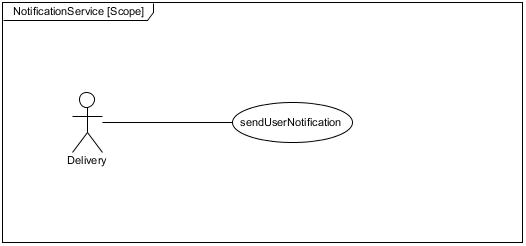
\includegraphics[width=1\textwidth]{./Pictures/UML/Usecase/NotificationServiceUseCase.jpg}\\[0cm]
	
	{\noindent}The scope of the NotificationService module includes
	\begin{itemize}
		\item Send a notification to the user to inform him/her of a potential delivery.
		\item Send a message to the local device to instruct delivery person.
		\item Set and get notification status.
	\end{itemize}
	
	\subsubsection{Domain Model}
	The domain model for the NotificationService module is shown below
	
	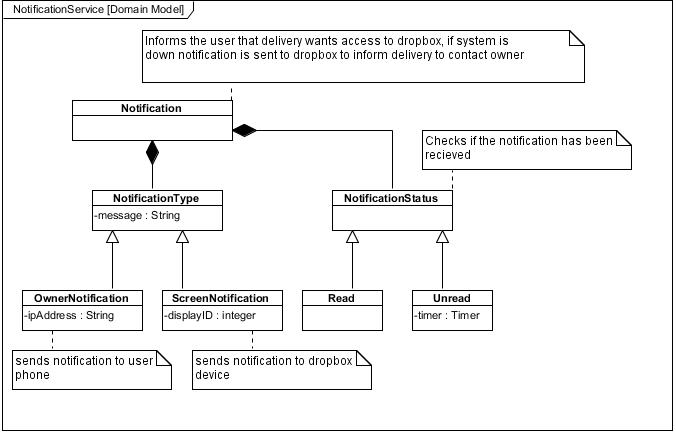
\includegraphics[width=1\textwidth]{./Pictures/UML/NotificationServiceDomain.jpg}\\[0cm]	
	
	{\noindent}
	
	\newpage
	\subsubsection{Use Cases}
	
	\begin{itemize}
		\item \textbf{sendUserNotification} - Will send a notification to the user, informing him/her of a delivery.\\[0.5cm]
		\textit{preconditions:}
		\begin{itemize}
			\item The alert button has been pressed.
			\item The home device is able to communicate with the server.
		\end{itemize}
		
		\textit{postconditions:}
		\begin{itemize}
			\item A notification is sent to the user.\\[0.5cm]
		\end{itemize}
		
		\item \textbf{sendLocalNotification} -  Will generate a message that will be displayed on the local device.\\[0.5cm]
		\textit{preconditions:}
		\begin{itemize}
			\item The alert button has been pressed.
			\item The local device cannot communicate with the server.
		\end{itemize}
		
		\textit{postconditions:}
		\begin{itemize}
			\item A message is displayed on the local device interface.\\[0.5cm]
		\end{itemize}
		
		\item \textbf{setNotificationStatus} -  Allows the status of the sent notification to be set as Read, or Unread.\\[0.5cm]
		\textit{preconditions:}
		\begin{itemize}
			\item A notification has been sent.
		\end{itemize}
		
		\textit{postconditions:}
		\begin{itemize}
			\item The status of the notification is set to Unread. Once read it is set to red.\\[0.5cm]
		\end{itemize}
		
		\item \textbf{getNotificationStatus} -  Provides the user/system with the current status of the notification.\\[0.5cm]
		\textit{preconditions:}
		\begin{itemize}
			\item A notification status has been set.
		\end{itemize}
		
		\textit{postconditions:}
		\begin{itemize}
			\item Returns the status of the notification.\\[0.5cm]
		\end{itemize}
	\end{itemize}
\end{document}
